\documentclass{article}

\usepackage{url} 
\usepackage{geometry,afterpage}
\usepackage{pdfpages}
\usepackage{lastpage}
\usepackage{fancyhdr}
\usepackage{ngerman}
\usepackage{listings}

\usepackage{floatrow}
\usepackage[tableposition=top]{caption}
\floatsetup[table]{capposition=top}

\usepackage{amsmath, amssymb}

\usepackage[utf8]{inputenc}


\usepackage[numbib]{tocbibind}



\newcommand\twodigits[1]{%
   \ifnum#1<10 0#1\else #1\fi
}



\lhead{Plank'sches Wirkungsquantum}
\rhead{\today \\ J. Winkler}
%\cfoot{\twodigits{\thepage}~/ \pageref{LastPage}}
\cfoot{{\thepage}~/ \pageref{LastPage}}


\newcommand{\Ekin}{E_\text{kin}}

\begin{document}

\parindent0cm


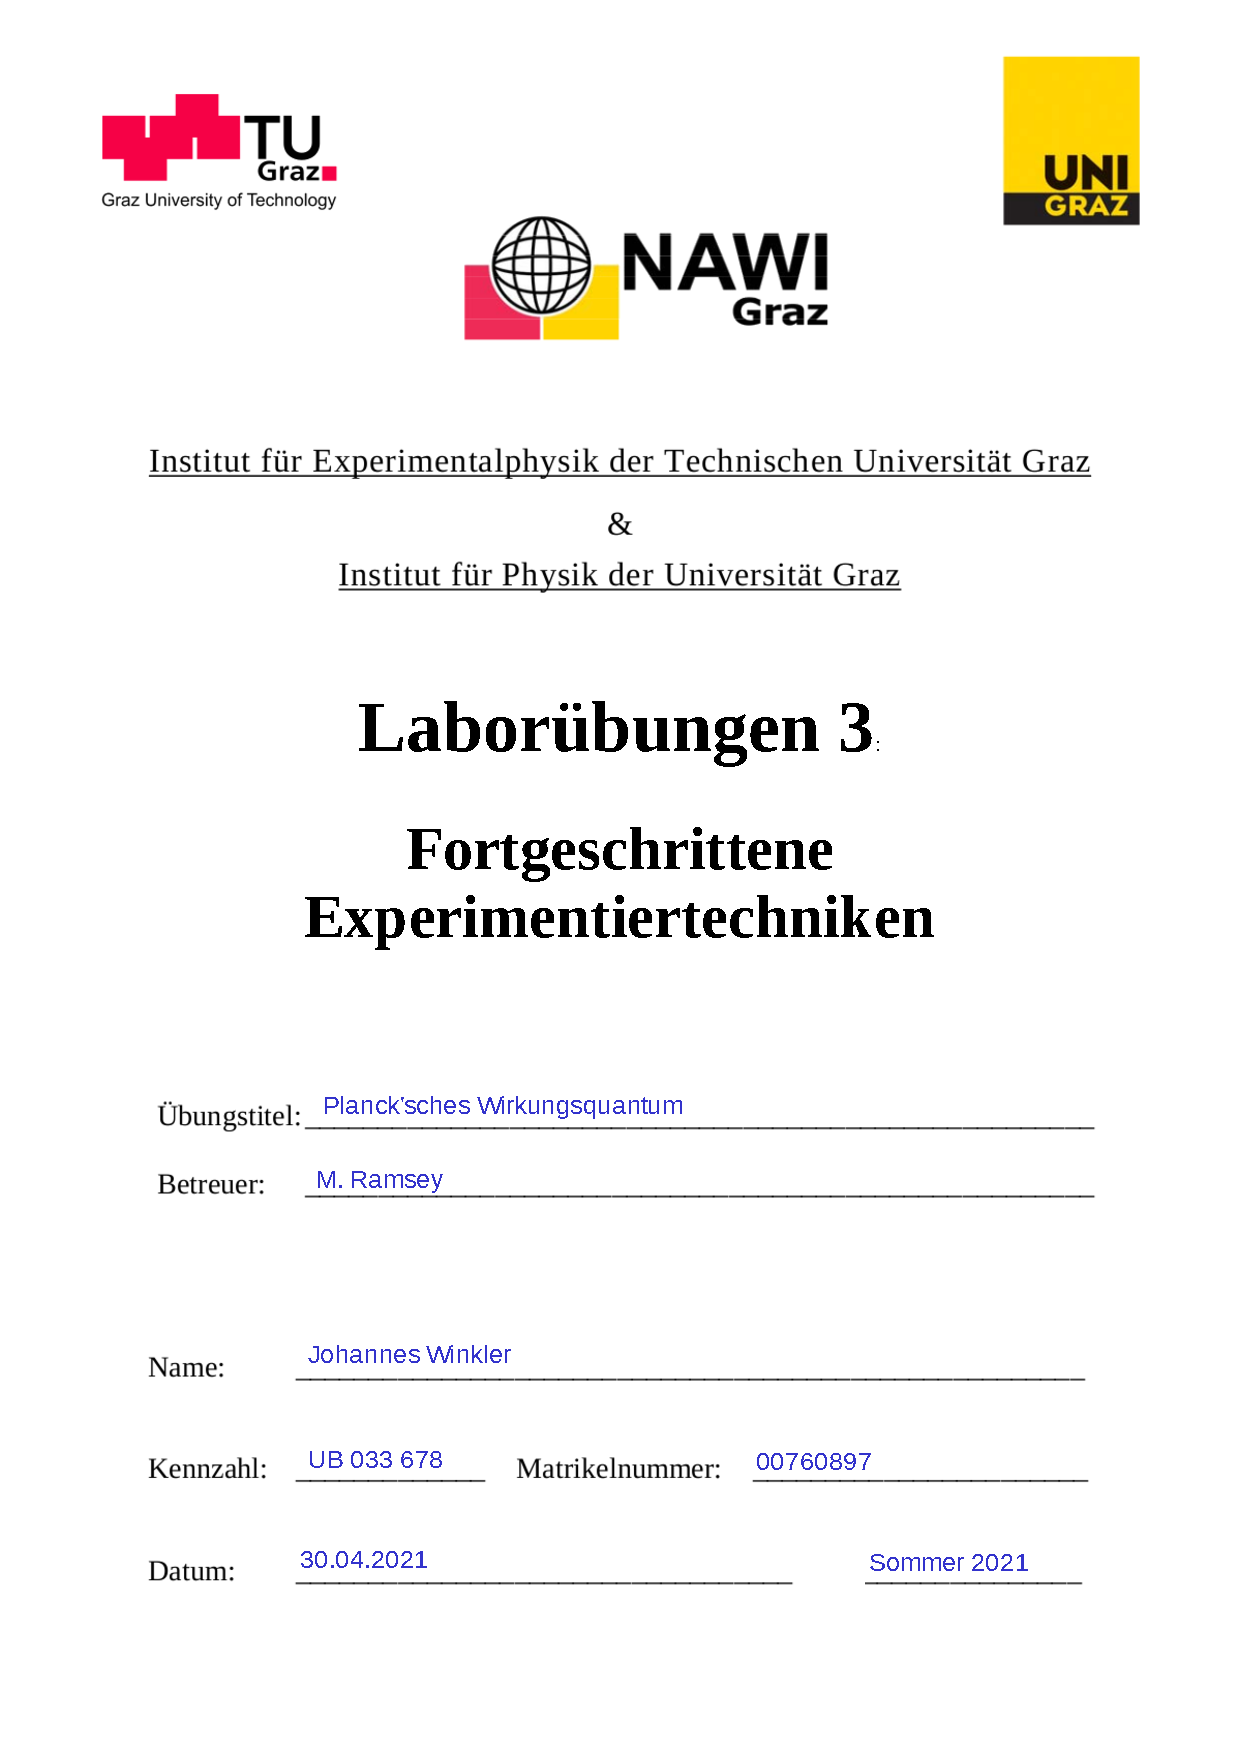
\includepdf{Deckblatt_neu_custom.pdf}

\tableofcontents
\newpage

\pagestyle{fancy}

\section{Aufgabenstellung}

Es muss die Austrittsarbeit $W$ und der numerische Wert des Planck'schen Wirkungsquantums mit Hilfe einer Vakuum-Photozelle bestimmt werden. 

\begin{figure}[H]
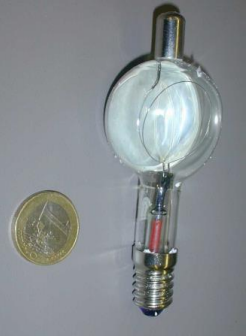
\includegraphics[scale=1.4]{versuch3.png}
\caption{Vakuum Photozelle. Quelle: \cite{moodle}}
\end{figure}

\section{Grundlagen}

Der Versuch basiert auf der Gleichung
\begin{align}
E = h\cdot \nu\label{eq:planck}
\end{align}
wobei $h$ das Planck'sche Wirkungsquantum ist. $E$ ist die Energie, eines Photons. Durch diese Gleichung kann man jedem Photon einer bestimmten Frequenz eindeutig eine Energie zuordnen. Die Konstante $h$ heißt Planck'sches Wirkungsquantum und ist gemäß \cite{wikipedia} festgesetzt als 
\begin{align}
h=6.62607015\cdot10^{34}~\text{Js}.
\end{align}
Der hier gegebene Wert ist seit 2019 exakt festgelegt und daher ohne Unsicherheit. Dieser Versuch sollte den Zahlenwert von $h$ näherungsweise bestimmen. 

~

Bei der Beleuchtung einer Photokathode mit kurzwelligem Licht einer bestimmten Frequenz $\nu$ werden Elektronen aus dem Material gelöst. Diese bilden einen Photostrom. Die Energie des Photons wird dabei in eine Austrittsarbeit (abhängig vom Material) und die kinetische Energie $\Ekin$ des gelösten Elektrons aufgeteilt. Insgesamt gilt für die Energiebilanz
\begin{align*}
h\cdot \nu = W + \Ekin
\end{align*}
wobei $W$ die Austrittsarbeit ist. Diese kann quasi als potenzielle Energie aufgefasst werden, die nötig ist, um ein Elektron aus dem Atomverband zu lösen.

Der Anteil der kinetischen Energie kann als Geschwindigkeit der Elektronen aufgefasst werden. Allerdings kann dieser auch in der Form 
\begin{align}
\Ekin = e\cdot U
\end{align}
dargestellt werden, wobei $U$ die Spannung zwischen Kathode und Anode und $e = 1.60217733 \cdot 10^{-19}$~C die Elementarladung ist. Dies wird durch eine Gegenspannung $U_G = -U$ realisiert. Diese Gegenspannung wird so lange variiert, bis der Photostrom zum erliegen kommt.




\begin{figure}[H]
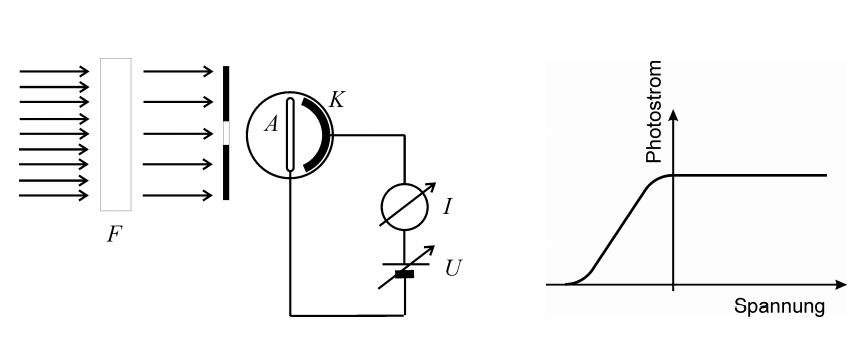
\includegraphics[scale=1.4]{versuch1.png}
\caption{Veranschaulichtes Grundprinzip des Messung des Experiments. Quelle: \cite{moodle}}
\end{figure}

Die Energie eines Photons ist einerseits durch Gleichung~\eqref{eq:planck} definiert, andererseits gilt wegen der Energieerhaltung
\begin{align}
h\cdot \nu = W + e\cdot U.
\end{align}
Das bedeutet, dass die Gesamtenergie des Photons in einen Anteil der Austrittsarbeit $W$ und in einen Spannungs-Anteil zerlegt wird.
Durch Umformen erhält man
\begin{align}
e\cdot U = k\cdot \nu - W \label{eq:regr_def1}
\end{align}
wobei hier durch eine lineare Regression die Koeffizienten bestimmt werden können. Man erhält die Steigung $k$ und den Achenabschnitt $d$. Insgesamt gilt 
\begin{align}
h &= k \\
W &= d
\end{align}
Wichtig an dieser Stelle ist, dass man die Austrittsarbeit in der Einheit Elektronenvolt erhält.


\newpage


\section{Versuchsaufbau}

Eine Quecksilber-Hochdruck-Dampflampe strahlt Licht in bestimmten Frequenzen. Dieses wird dann durch entsprechende Spaltblenden und Linsen auf ein Prisma gebündelt. Am Prisma wird der Lichtstrahl in ein Spektrum zerlegt. Durch den drehbaren Spiegel und einer Spaltblende kann man dann einen bestimmten Teil des Spektrums selektieren und dann mit einer bestimmten Frequenz die Photozelle beleuchten. Diese Photozelle erzeugt nun einen Photostrom, der für die weiteren Messungen verwendet wird.

\begin{figure}[H]
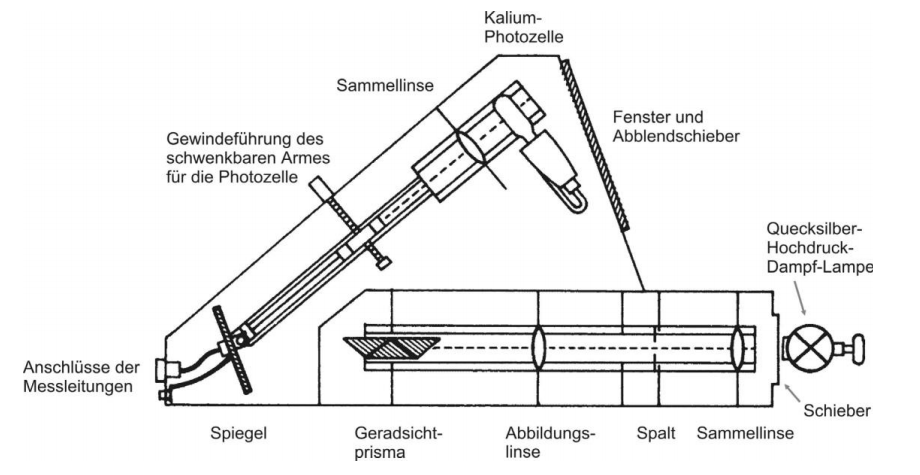
\includegraphics[scale=1.6]{versuch2.png}
\caption{Versuchsaufbau mit Erklärung. Quelle: \cite{moodle}}
\label{fig:versuch2}
\end{figure}


\section{Geräteliste}


\begin{table}[H]
\caption{Liste der verwendeten Geräte}
~
\begin{tabular}{l|l}
 & Geräte  \\
\hline
1 & Spektrometeraufbau mit Geradsichtprisma und Photozelle  \\
2 & Lichtquelle: Quecksilber-Hochdruck-Dampf-Lampe  \\
3 & Messverstärker \\
4 &  Multimeter, div. Kabel.
\end{tabular}

\end{table}

\newpage

\section{Durchführung und Messergebnisse}

Zuerst wird die Hg-Hochdruck-Dampflampe eingeschalten. Dann wird der drehbare Spiegel angepasst, sodass die Photozelle mit ausgewählten Spektrallinien bestrahlt werden kann.
\begin{table}[H]
\caption{Wellenlängen und Frequenzen der zu messenden Spektrallinien.}
\begin{tabular}{ccc}
Wellenlänge $\lambda$ / nm & Frequenz $\nu$ / Hz & Farbe \\
\hline
578 & $5.19 \cdot 10^{14}$ & gelb \\
546 & $5.49 \cdot 10^{14}$ & grün \\
493 & $6.08 \cdot 10^{14}$ & cyan \\
436 & $6.88 \cdot 10^{14}$ & blau \\
405 & $7.41 \cdot 10^{14}$ & violett
\end{tabular}
\end{table}

Die Messungen werden für alle 5 Spektrallinien durchgeführt. Dabei ist zu achten, dass die Abdeckung des Versuchs geschlossen ist. Es wird die für jede Wellenlänge die Gegenspannung variiert um, den Nulldurchgang zu finden. Der Photostrom wird als Spannung gemessen, diese ist dann proportional zum Strom. Der genaue Messwiderstand ist nicht bekannt. Da aber ohnehin nur der Nulldurchgang benötigt wird, ist der Proportionalitätsfaktor zwischen Photostrom und Photospannung nicht relevant.

Zuerst wurde eine betragsmäßig sehr hohe Gegenspannung (-3 Volt) eingestellt, sodass kein Photostrom fließt. Der Wert am Voltmeter der Photospannung (je nach Spektrallinie zwischen 0.15 und 0.32~mV) wurde als Nullpunkt festgesetzt. Dann wurde die Gegenspannung von -3~V auf 0~V erhöht und die relevanten Messdaten für Kurve zwischen Gegenspannung und Photostrom dokumentiert.

Das Experiment wird für alle Spektralfarben wiederholt.


\newpage
\begin{figure}[H]
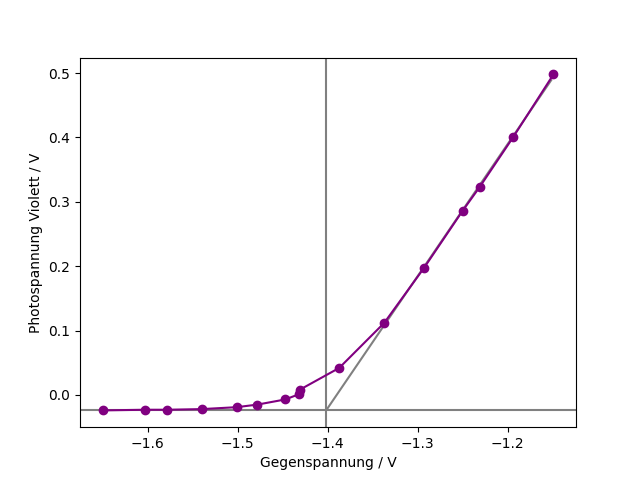
\includegraphics[scale=0.6]{purple.png}
\caption{Gemessener Photostrom (als Spannung) bei violettem Licht in Abhängigkeit der Gegenspannung. Geschätzter Nulldurchgang ist mit vertikaler Linie markiert.}
\label{fig:daten_purple}
\end{figure}
\begin{figure}[H]
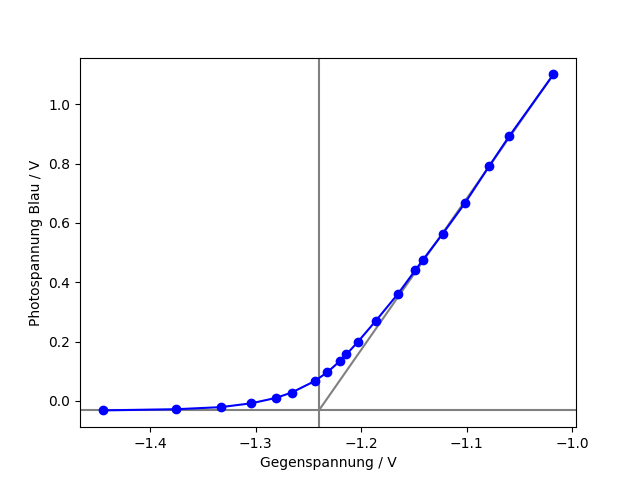
\includegraphics[scale=0.6]{blue.png}
\caption{Gemessener Photostrom (als Spannung) bei blauem Licht in Abhängigkeit der Gegenspannung. Geschätzter Nulldurchgang ist mit vertikaler Linie markiert.}
\label{fig:daten_blue}
\end{figure}

\newpage
\begin{figure}[H]
 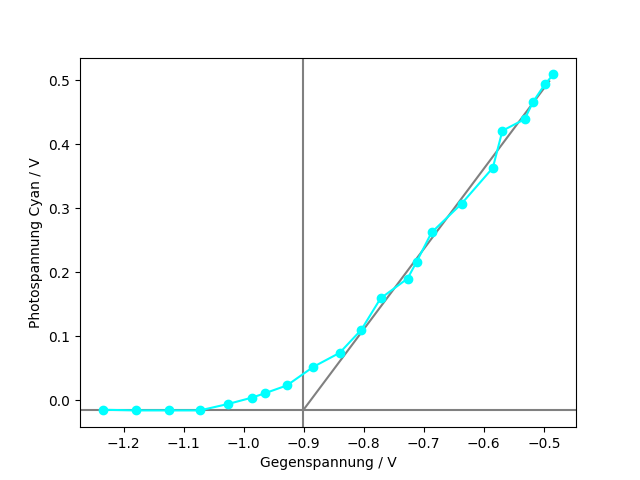
\includegraphics[scale=0.6]{cyan.png}
\caption{Gemessener Photostrom (als Spannung) bei blaugrünem Licht in Abhängigkeit der Gegenspannung. Geschätzter Nulldurchgang ist mit vertikaler Linie markiert.}
\label{fig:daten_cyan}
\end{figure}
\begin{figure}[H]
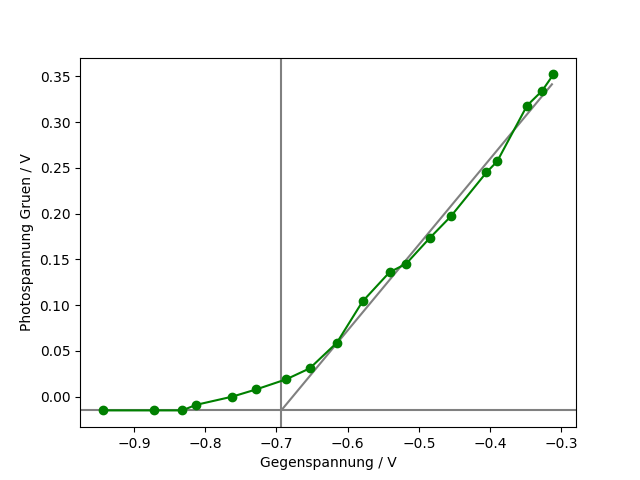
\includegraphics[scale=0.6]{green.png}
\caption{Gemessener Photostrom (als Spannung) bei grünem Licht in Abhängigkeit der Gegenspannung. Geschätzter Nulldurchgang ist mit vertikaler Linie markiert.}
\label{fig:daten_green}
\end{figure}
\newpage
\begin{figure}[H]
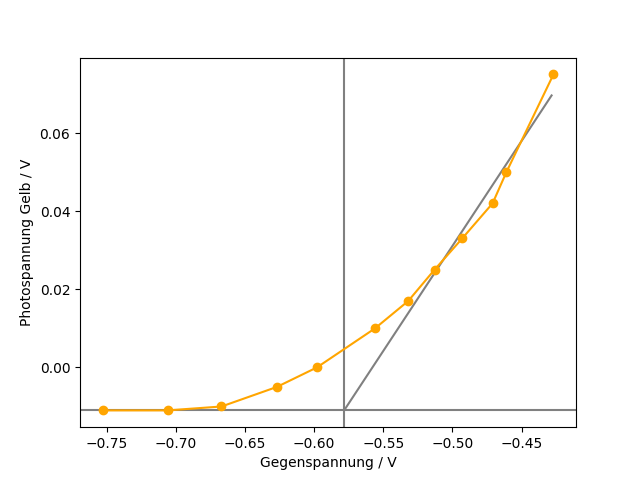
\includegraphics[scale=0.6]{orange.png}
\caption{Gemessener Photostrom (als Spannung) bei gelbem Licht in Abhängigkeit der Gegenspannung. Geschätzter Nulldurchgang ist mit vertikaler Linie markiert.}
\label{fig:daten_yellow}
\end{figure}
\newpage



\section{Auswertung}

In den Grafiken~\ref{fig:daten_purple} bis \ref{fig:daten_yellow} wurden die Messwerte eingezeichnet. Dann wurde aufgrund der Daten ein Nulldurchgang berechnet. Dazu wurde die Kurve \textit{per Augenmaß} in einen flachen und einen linearen Teil zerlegt. Im linearen Teil wurde mit Hilfe einer Regressionsgeraden der Nulldurchgang ermittelt. Der Nulldurchgang ist nach Frequenz aufgeschlüsselt in Tabelle~\ref{tab:null} zusammengefasst.

Die Bestimmung der Unsicherheiten gestaltet sich schwierig. Zum einen ist die Spaltblende zur Selektion eines Teils des Spektrums nicht beliebig dünn, daher werden mehrere Lichtfrequenzen auf die Photozelle übertragen. Zum anderen kann eine minimale Änderung der Lichtverhältnisse zu einer Verfälschung der Daten führen. Da zwischen grünem und gelben Licht ein Unterschied von $0.30\cdot 10^{14}$~Hz ist, wird als Unsicherheit $\Delta \nu = 0.10\cdot 10^{14}~$Hz geschätzt. Für die Stoppspannung ist eine Unsicherheit von $\Delta U_S = 0.1000~$V sinnvoll, da aufgrund des kontinuierlichen Anstiegs keine genauere Aussage über den Nulldurchgang möglich ist.

\begin{table}[H]
\caption{Stoppspannung $U_S$ je nach Frequenz $\nu$.}
\begin{tabular}{l|r|r}
Farbe & $\nu$ / $10^{14}$~Hz  & $U_S$ / V \\
\hline
Violett & 7.41 & 1.402\\
Blau & 6.88 & 1.240\\
Cyan & 6.08 & 0.901\\
Gruen & 5.49 & 0.693\\
Gelb & 5.19 & 0.578\\

\end{tabular}
\label{tab:null}
\end{table}


\begin{figure}[H]
\center
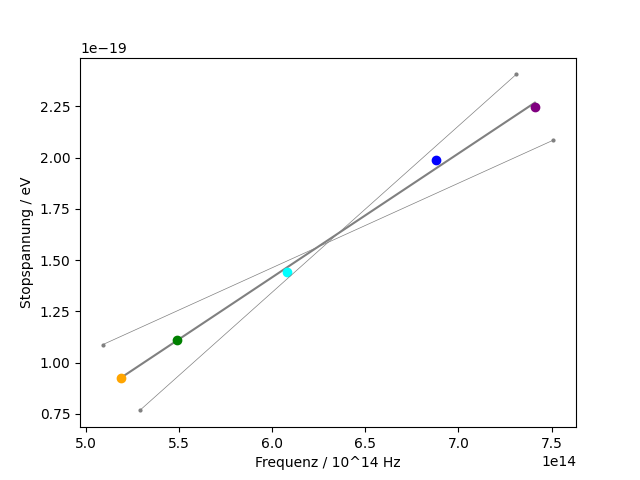
\includegraphics[scale=0.7]{regression.png}
\caption{Stoppspannung in Abhängigkeit von der Frequenz und mögliche Abweichungen der Steigung für die Fehlerrechnung.}
\label{fig:stopspannung_regression}
\end{figure}
In Abbildung~\ref{fig:stopspannung_regression} sieht man eine Regressionsgerade der Form $e\cdot U = k\cdot \nu + d$ mit den Koeffizienten
\begin{align*}\\
k &= 6.043\cdot 10^{-34}~\text{Js}\\
d &= -2.210\cdot 10^{-19}~\text{J}
\\\end{align*}

Gemäß Gleichung~\eqref{eq:regr_def1} kann die Regressionsgerade auch als 
\begin{align*}
e\cdot U = h\cdot \nu - W
\end{align*}
geschrieben werden. Als Fehlerrechnung für $k$ kann man die Steigung zwischen den beiden \textit{äußeren Punkten} (also Violett und Gelb) verwenden, wobei die Koordinaten mit der gegebenen Unsicherheit behaftet sind. Grafisch sieht man das in Abbildung~\ref{fig:stopspannung_regression}.
\begin{align*}
\Delta k = \frac{e}{2}\cdot\left( \frac{ U_S(\text{violett}) - U_S(\text{gelb}) + 2\cdot \Delta U_S}{\nu(\text{violett}) - \nu(\text{gelb})- 2\cdot \Delta \nu} - \frac{ U_S(\text{violett} - 2\cdot \Delta \nu) - U_S(\text{gelb}) - 2\cdot \Delta U_S}{\nu(\text{violett}) - \nu(\text{gelb}) + 2\cdot \Delta \nu}\right)
\end{align*}



Daraus ergeben sich für das Planck'sche Wirkungsquantum und die Austrittsarbeit die Werte
\begin{align*}
R_H &= (5.46 \pm 0.06)\cdot 10^{-3} ~\text{m}^3/\text{C} \\
p &= (114\pm1) \cdot 10^{19} ~\text{m}^{-3}
\end{align*}




\section{Diskussion}

Die Messergebnisse können dadurch verfälscht werden, dass der Spiegel bei der Abdeckung des Versuchaufbaus sich leicht verstellen kann. Außerdem ist die Wahl der Frequenz durch \textit{Augenmaß} bestimmt, da die Farbbereiche des Spektrums nicht eindeutig abgegrenzt werden können. Außerdem ist der Bereich \textit{cyan} in der Praxis relativ schwer zu erkennen. Deswegen ist gerade bei diesem Wert darauf zu achten, dass es kein Ausreisser ist. Eine kleine Abweichung der Farbe ist eine große Abweichung in der Frequenz. Das macht es auch relativ schwer, die Unsicherheiten zu bestimmen. Diese können nur geschätzt werden.

\section{Zusammenfassung}

Als Ergebnis erhält man
\begin{align*}
R_H &= (5.46 \pm 0.06)\cdot 10^{-3} ~\text{m}^3/\text{C} \\
p &= (114\pm1) \cdot 10^{19} ~\text{m}^{-3}
\end{align*}
wobei $h$ dem Literaturwert entspricht (vergleiche dazu \cite{wikipedia}). Da die Austrittsarbeit materialabhängig ist, kann man hier keinen Wert zum Vergleichen finden.


\begin{thebibliography}{9}
\bibitem{moodle} S. Surnev: Skript zum Plank'schen Wirkungsquantum aus dem Moodle der Karl-Franzens Universität, Institut für Physik, 30.04.2021.
\bibitem{messmethoden}  R. Dämon: Einführung in die physikalischen Messmethoden, Graz 2016.
\bibitem{wikipedia} \url{https://www.bipm.org/en/measurement-units}, 30.04.2021, 21:30.
\bibitem{regression} \url{https://de.wikipedia.org/wiki/Lineare_Einfachregression}, 30.04.2021, 22:30.
\bibitem{python} Python-Skript zur Berechnung der Daten, zur Visualisierung und zum Generieren von \LaTeX-Code für diesen Bericht.
\end{thebibliography}


\newpage 
%\appendix
%\section{Python Skript}



\definecolor{commentgreen}{RGB}{2,112,10}
\definecolor{eminence}{RGB}{108,48,130}
\definecolor{weborange}{RGB}{255,165,0}
\definecolor{frenchplum}{RGB}{129,20,83}

\lstdefinelanguage{python}{
    morekeywords={def, for, range, abs, return},
    otherkeywords={<-,->, |>, \%\{, \}, \{, \, (, )},
    sensitive=true,
    morecomment=[l]{\#},
    morecomment=[n]{/*}{*/},
    morecomment=[s][\color{purple}]{:}{\ },
    morestring=[s][\color{orange}]"",
    commentstyle=\color{commentgreen},
    keywordstyle=\color{eminence},
    stringstyle=\color{red},
	basicstyle=\ttfamily,
	breaklines,
	showstringspaces=false,
	frame=tb
}
%\lstinputlisting[language=Python,captionpos=b, label=lst:test,caption={Auswertung}]{script.py}

%\lstinputlisting[language=Python,captionpos=b, label=lst:test,caption={Bessel Auswertung}]{generate_numbers_bessel.py}



\end{document}